%% This template can be used to write a paper for
%% Computer Physics Communications using LaTeX.
%% For authors who want to write a computer program description,
%% an example Program Summary is included that only has to be
%% completed and which will give the correct layout in the
%% preprint and the journal.
%% The `elsarticle' style is used and more information on this style
%% can be found at 
%% http://www.elsevier.com/wps/find/authorsview.authors/elsarticle.
%%
%%
%%\documentclass[preprint,12pt]{elsarticle}

%% Use the option review to obtain double line spacing
%% \documentclass[preprint,review,12pt]{elsarticle}

%% Use the options 1p,twocolumn; 3p; 3p,twocolumn; 5p; or 5p,twocolumn
%% for a journal layout:
%% \documentclass[final,1p,times]{elsarticle}
%% \documentclass[final,1p,times,twocolumn]{elsarticle}
%% \documentclass[final,3p,times]{elsarticle}
%% \documentclass[final,3p,times,twocolumn]{elsarticle}
%% \documentclass[final,5p,times]{elsarticle}
\documentclass[final,5p,times,twocolumn]{elsarticle}

%% if you use PostScript figures in your article
%% use the graphics package for simple commands
%% \usepackage{graphics}
%% or use the graphicx package for more complicated commands
\usepackage{graphicx}
%% or use the epsfig package if you prefer to use the old commands
%% \usepackage{epsfig}

%% The amssymb package provides various useful mathematical symbols
\usepackage{amssymb}
%% The amsthm package provides extended theorem environments
%% \usepackage{amsthm}

%% The lineno packages adds line numbers. Start line numbering with
%% \begin{linenumbers}, end it with \end{linenumbers}. Or switch it on
%% for the whole article with \linenumbers after \end{frontmatter}.
\usepackage{lineno}

%% natbib.sty is loaded by default. However, natbib options can be
%% provided with \biboptions{...} command. Following options are
%% valid:

%%   round  -  round parentheses are used (default)
%%   square -  square brackets are used   [option]
%%   curly  -  curly braces are used      {option}
%%   angle  -  angle brackets are used    <option>
%%   semicolon  -  multiple citations separated by semi-colon
%%   colon  - same as semicolon, an earlier confusion
%%   comma  -  separated by comma
%%   numbers-  selects numerical citations
%%   super  -  numerical citations as superscripts
%%   sort   -  sorts multiple citations according to order in ref. list
%%   sort&compress   -  like sort, but also compresses numerical citations
%%   compress - compresses without sorting
%%
\biboptions{comma,square}

% \biboptions{}

%% This list environment is used for the references in the
%% Program Summary
%%
\newcounter{bla}
\newenvironment{refnummer}{%
\list{[\arabic{bla}]}%
{\usecounter{bla}%
 \setlength{\itemindent}{0pt}%
 \setlength{\topsep}{0pt}%
 \setlength{\itemsep}{0pt}%
 \setlength{\labelsep}{2pt}%
 \setlength{\listparindent}{0pt}%
 \settowidth{\labelwidth}{[9]}%
 \setlength{\leftmargin}{\labelwidth}%
 \addtolength{\leftmargin}{\labelsep}%
 \setlength{\rightmargin}{0pt}}}
 {\endlist}

\journal{Computer Physics Communications}

%% Extra stuff by DLG

\usepackage{amsmath,mathtools}
\usepackage{hyperref}
\usepackage{xspace}
\usepackage{dirtree}
\usepackage{listings}
\usepackage{color}

\definecolor{mygreen}{rgb}{0,0.6,0}
\definecolor{mygray}{rgb}{0.5,0.5,0.5}
\definecolor{mymauve}{rgb}{0.58,0,0.82}

\lstset{ %
  backgroundcolor=\color{white},   % choose the background color; you must add \usepackage{color} or \usepackage{xcolor}; should come as last argument
  basicstyle=\footnotesize,        % the size of the fonts that are used for the code
  breakatwhitespace=false,         % sets if automatic breaks should only happen at whitespace
  breaklines=true,                 % sets automatic line breaking
  captionpos=b,                    % sets the caption-position to bottom
  commentstyle=\color{mygreen},    % comment style
  deletekeywords={...},            % if you want to delete keywords from the given language
  escapeinside={\%*}{*)},          % if you want to add LaTeX within your code
  extendedchars=true,              % lets you use non-ASCII characters; for 8-bits encodings only, does not work with UTF-8
  frame=single,                       % adds a frame around the code
  keepspaces=true,                 % keeps spaces in text, useful for keeping indentation of code (possibly needs columns=flexible)
  keywordstyle=\color{blue},       % keyword style
  language=Octave,                 % the language of the code
  morekeywords={*,...},           % if you want to add more keywords to the set
  numbers=left,                    % where to put the line-numbers; possible values are (none, left, right)
  numbersep=5pt,                   % how far the line-numbers are from the code
  numberstyle=\tiny\color{mygray}, % the style that is used for the line-numbers
  rulecolor=\color{black},         % if not set, the frame-color may be changed on line-breaks within not-black text (e.g. comments (green here))
  showspaces=false,                % show spaces everywhere adding particular underscores; it overrides 'showstringspaces'
  showstringspaces=false,          % underline spaces within strings only
  showtabs=false,                  % show tabs within strings adding particular underscores
  stepnumber=2,                    % the step between two line-numbers. If it's 1, each line will be numbered
  stringstyle=\color{mymauve},     % string literal style
  tabsize=2,                       % sets default tabsize to 2 spaces
  title=\lstname                   % show the filename of files included with \lstinputlisting; also try caption instead of title
}

\let\oldhat\hat
\renewcommand{\vec}[1]{\mathbf{#1}}
\renewcommand{\hat}[1]{\oldhat{\mathbf{#1}}}
\newcommand{\kpar}{\ensuremath{k_{\parallel}}\xspace}
\newcommand{\vth}{\ensuremath{v_{\mathrm{th}}}\xspace}
\newcommand{\kj}{\textsc{Kinetic-j}\xspace}
\newcommand{\fdfd}{\textsc{fdfd}\xspace}
\newcommand{\aorsa}{\textsc{aorsa}\xspace}
\newcommand{\toric}{\textsc{toric}\xspace}
\newcommand{\jp}{\ensuremath{\vec{j}_{\mathrm{1}}}\xspace}
\newcommand{\E}{\ensuremath{\vec{E}_{\mathrm{1}}}\xspace}
\newcommand{\jpc}{\ensuremath{\vec{j}_{\mathrm{1}}^{\mathrm{c}}\left(\vec{r},t\right)}\xspace}
\begin{document}

\begin{frontmatter}

%% Title, authors and addresses

%% use the tnoteref command within \title for footnotes;
%% use the tnotetext command for the associated footnote;
%% use the fnref command within \author or \address for footnotes;
%% use the fntext command for the associated footnote;
%% use the corref command within \author for corresponding author footnotes;
%% use the cortext command for the associated footnote;
%% use the ead command for the email address,
%% and the form \ead[url] for the home page:
%%
%% \title{Title\tnoteref{label1}}
%% \tnotetext[label1]{}
%% \author{Name\corref{cor1}\fnref{label2}}
%% \ead{email address}
%% \ead[url]{home page}
%% \fntext[label2]{}
%% \cortext[cor1]{}
%% \address{Address\fnref{label3}}
%% \fntext[label3]{}

\title{\kj: A computational kernel for calculating the linear, kinetic, configuration space plasma current for time harmonic wave electric fields.}

%% use optional labels to link authors explicitly to addresses:
%% \author[label1,label2]{<author name>}
%% \address[label1]{<address>}
%% \address[label2]{<address>}

\author[a]{David L. Green\corref{author}}
\author[a,b]{Lee A. Berry}
\author[b]{Adam B. Simpson}
\author[a,c]{T.R. Younkin}

\cortext[author] {Corresponding author.\\\textit{E-mail address:} greendl1@ornl.gov}
\address[a]{Oak Ridge National Laboratory, 1 Bethel Valley Rd., Oak Ridge, Tennessee 37831, USA}
\address[b]{XCEL Engineering, 1066 Commerce Park Dr., Oak Ridge, Tennessee 37830, USA}
\address[c]{Universtity of Tennessee, Knoxville, Tennessee 37996, USA}

\begin{abstract}
%% Text of abstract
We present the \kj code, a computational kernel for evaluating the linear kinetic plasma response to an applied time harmonic wave electric field. This code addresses the need for a configuration space evaluation of the the plasma current to enable kinetic full-wave solvers for waves in hot plasmas to move beyond the limitations of the traditional Fourier spectral methods. We benchmark the kernel via comparison with the standard $\vec{k}$-space forms of the hot plasma conductivity tensor. 
\end{abstract}

\begin{keyword}
%% keywords here, in the form: keyword \sep keyword
Plasma; conductivity; linear; kinetic; hot; configuration space.

\end{keyword}

\end{frontmatter}

%%
%% Start line numbering here if you want
%%
\linenumbers

% Computer program descriptions should contain the following
% PROGRAM SUMMARY.

{\bf PROGRAM SUMMARY}
  %Delete as appropriate.

\begin{small}
\noindent
{\em Program Title:} \kj                           \\
{\em Licensing provisions: }MIT                             \\
{\em Programming language: }C++ / IDL / CUDA                 \\
%{\em Supplementary material:}                                 \\
  % Fill in if necessary, otherwise leave out.
%{\em Journal reference of previous version:}                  \\
  %Only required for a New Version summary, otherwise leave out.
%{\em Does the new version supersede the previous version?:}   \\
  %Only required for a New Version summary, otherwise leave out.
%{\em Reasons for the new version:}\\
  %Only required for a New Version summary, otherwise leave out.
%{\em Summary of revisions:}*\\
  %Only required for a New Version summary, otherwise leave out.
{\em Nature of problem: }Configuration space evalution of the linear, kinetic plasma current.\\
  %Describe the nature of the problem here. \\
{\em Solution method: }Direct numerical evaluation of the linearized solution of the Vlasov equation, i.e., provided a time harmonic wave electric field as input, evalutate the unperturbed Lorentz orbit of each phase-space (position and velocity) point trajectory and integrate over its time history, then take the first velocity moment to calculate current.\\
  %Describe the method solution here.
{\em Additional comments:} This initial version is 1x-3v, and accepts input fields in either Cartesian or cylindrical coordinates. The code is hosted at \url{https://github.com/ORNL-Fusion/kineticj}.\\
  %Provide any additional comments here.
%   \\ 
%\begin{thebibliography}{0}
%\bibitem{1}Reference 1         % This list should only contain those items referenced in the                 
%\bibitem{2}Reference 2         % Program Summary section.   
%\bibitem{3}Reference 3         % Type references in text as [1], [2], etc.
%                               % This list is different from the bibliography at the end of 
%                               % the Long Write-Up.
%\end{thebibliography}
%* Items marked with an asterisk are only required for new versions
%of programs previously published in the CPC Program Library.\\
\end{small}
%
%% main text
\section{Introduction}
\label{section:introduction}
The application of megawatts of radio frequency (RF) power in the ion-cyclotron, lower-hybrid, and electron-cyclotron range of frequencies is often required for heating and current drive applications in magnetically confined fusion plasmas. The extreme environment, as well as the large range of space and time scales of the relevant physics mean that predicting how a hot (several keV), magnetically confined plasma will respond to applied RF power has relied heavily on high performance computing. Here we present a computational kernel which provides this kinetic response, i.e., the plasma current $\vec{j}$; hence the name \kj.  
%

The hot nature of fusion plasmas means kinetic (non-local / velocity space) effects require a wave vector dependent conductivity tensor $\bar{\sigma}\left(\omega,\vec{k}\right)$ (in addition to the frequency $\omega$ dependence for the cold / local approximation) \cite[cf.,][]{stix,fukuyama1986}. Traditional methods for calculating the linear, kinetic (hot) full wave plasma response (current) rely on a spectral method \cite[e.g.,][]{brambilla1999,jaeger2001,jaeger2002a}, i.e., a spatial Fourier transform of the time harmonic form of Maxwell's equations (Helmholtz wave equation) such that the $\vec{k}$ dependent conductivity fits naturally within the numerical method. Examples of such implementations are the All-ORders Spectral Algorithm (AORSA) \cite{jaeger2003a}, and TORIC \cite{brambilla1999,wright2004}. These methods have seen much success in application to the well confined core plasma of tokamaks in 2 spatial dimensions (in cylindrical coordinates; $r$ (radial) and $z$ (vertical), with $\mathrm{exp}\left(in\phi\right)$ Fourier decomposition in toroidal angle $\phi$, where $n$ is the toroidal mode number), with some limited application in real 3D \cite[c.f. Fig.~8 of][]{jaeger2002a}. 

However, recent efforts \cite[e.g.,][]{bertelli2014,wright2015,jenkins2015} to move toward quantitative prediction of high power RF antenna designs for fusion applications has meant a requirement of resolving the geometric details of the antenna and other plasma facing surfaces. The Fourier spectral method is ill-suited to such problems where there are no periodic coordinates (i.e., field lines intersecting the walls), or surfaces aligned with coordinate directions. The typical approach to this problem of quantitative prediction where both the geometric fidelity of the antenna and surrounds must be resolved, in addition to the hot plasma kinetics, is to couple a spectral solver for the core plasma, and a cold-plasma representation (no $\vec{k}$ dependence in the conductivity, and therefore no advantage for the Fourier spectral method so geometry conforming methods such as the finite element methods may be applied). These approaches have seen some success. However, they are still limited by several fundamental restrictions of the Fourier spectral method. These include the numerical limitations of uniform resolution in any spectral direction, matrices approaching dense (or indeed fully dense for the approach of AORSA), and $N^3$ work scaling to invert such dense matrices, as well as physics limitations including the stationary-phase approximation \cite{stix,brambilla}.  

An alternative approach to coupling core spectral, and boundary finite element full-wave solvers was presented by \cite{green2014} where the computational power of modern computing architectures was leveraged in an operator-split, iterative approach to the inclusion of kinetic effects to existing cold-plasma full-wave solvers. That paper was the proof of principle for parallel kinetic effects. This is similar to, although extended beyond, the work of \cite{meneghini2009,shiraiwa2010a} where the damping term for configuration space finite element method LH full-wave calculations was added iteratively. Here we present the full computational kernel for evaluating both the propagation and damping components of the kinetic plasma current, with verification benchmarks showing the capability for both parallel and perpendicular kinetic effects. It is also straight forward to conceive an approach where such a kernel is embedded within the matrix construction step of a finite element or similar method, as was done by \cite{svidzinski2016}. However, such an approach will still produce partially dense matrices, such that when moving to the 3D problems of interest, the block sparsity pattern may result in scaling difficulties which may limit utilizing the full power of leadership class computing platforms. The operator-split approach of \cite{green2014} trades the advantages of a diagonal dielectric tensor for the challenge of convergence on the iteration.    

In the remainder of the paper, section~\ref{section:model} describes the model evaluated by the code, section~\ref{section:implementation} describes the numerical implementation, section~\ref{section:program} details running the program, section~\ref{section:verification} presents the benchmark cases for verification, section~\ref{section:performance} covers program performance, and lastly we discuss future work in section~\ref{section:discussion}.
%
\section{Model}
\label{section:model}
%
In the operator split, iterative approach of \cite{green2014}, the wave electric field is known from an initial guess at the plasma current, i.e., a cold-plasma full-wave solution. Provided this, or any time harmonic, complex valued wave electric field $\vec{E}_{\mathrm{1}}\left(\vec{r},t\right)=\vec{E}_{\mathrm{1}}\left(\vec{r}\right)\exp{\left(-i\omega t\right)}$, the \kj kernel evaluates the following expressions (the second operator $\mathfrak{L}_{\mathrm{2}}$ in the splitting of \cite{green2014}) to provide the kinetic plasma current \jp for that $\vec{E}_{\mathrm{1}}\left(\vec{r}\right)$.

\begin{linenomath}
\begin{equation}
\jp=\mathfrak{L}_{\mathrm{2}}\vec{E}_{\mathrm{1}}=q\int \vec{v}f_{\mathrm{1}}\left(\vec{r},\vec{v},t\right)d\vec{v}
\label{eq:j1}
\end{equation}
\end{linenomath}

The kinetic constituative relation is determined by solving for the oscillating piece ($f_{\mathrm{1}}$) of the distribution function $f\left(\vec{r},\vec{v},t\right)=f_{\mathrm{0}}\left(\vec{r},\vec{v}\right)+f_{\mathrm{1}}\left(\vec{r},\vec{v},t\right)$ which satisfies the linearized Vlasov equation as 
%
%\begin{widetext}
\begin{linenomath}
\begin{equation}
\begin{split}
\label{eq:lin_vlasov}
\frac{df_1}{dt}=&\frac{\partial f_1}{\partial t}+\vec{v}\cdot\nabla f_{\mathrm{1}}+\frac{q}{m}\left(\vec{v}\times\vec{B}_{\mathrm{0}}\right)\cdot\nabla_v f_1\\=&-\frac{q}{m}\left(\vec{E}_1+\vec{v}\times\vec{B}_1\right)\cdot\nabla_v f_0
\end{split}
\end{equation}
\end{linenomath}
%\end{widetext}
%
By the method-of-characteristics, and with an initial condition as $f_{\mathrm{1}}\left(t=-\mathrm{\infty}\right)=0$, $f_{\mathrm{1}}$ is 
%
%\begin{widetext}
\begin{linenomath}
\begin{equation}
\begin{split}
\label{eq:f1}
f_{\mathrm{1}}\left(\vec{r},\vec{v},t\right)=-\frac{q}{m}\int_{-\mathrm{\infty}}^{t}
\Big(\vec{E}_{\mathrm{1}}\left(\vec{r}',t'\right)+\vec{v}\left(t'\right)\\ \times\vec{B}_1\left(\vec{r}',t'\right) 
\hspace{0cm}\Big) \cdot\nabla_{v'} f_{\mathrm{0}} \left(\vec{r}',\vec{v}',t'\right)dt'
\end{split}
\end{equation}
\end{linenomath}
%\end{widetext}
%
where the characteristic curves $\left(\vec{r}',\vec{v}',t'\right)$ are given by the unperturbed particle trajectories
%
\begin{linenomath}
\begin{equation}
\begin{split}
\label{eq:trajectories}
\frac{d\vec{r}'}{dt'}&=\vec{v}'\\
\frac{d\vec{v}'}{dt'}&=\frac{q}{m}\left(\vec{v}'\times\vec{B}_{\mathrm{0}}\left(\vec{r}'\right)\right)
\end{split}
\end{equation}
\end{linenomath}

%need to add final condition for r and v at t' = t
Evaluating $\jp$ in this way as the integration along unperturbed, configuration-space particle trajectories yields several advantages beyond extending a cold-plasma solver to include kinetics. While the the driving motivation for this work is the need to solve higher fidelity problems (which include kinetic effects only in some part of the domain, but also exhibit variable spatial scales) than is presently possible with present spectral approaches (as represented by the first two of the following items) our approach will also address the following additional issues present in traditional methods. 
%
\begin{itemize}
\item{Compatible with variable mesh resolution.}
\item{Improved algorithmic scaling, i.e., access problems with more degrees of freedom such as real-3D.}
\item{No requirement on field aligned grids.}
\item{Includes violations of stationary phase approximation (i.e., upshift of the wave-number along particle trajectories \cite[]{berry2016})}
\item{Produces sparse, banded tri-diagonal matrices via a diagonal dielectric tensor.}
\end{itemize}
%
The last of these items has implications for the scalability of the auxiliary full-wave solver.
%
\section{Numerical Implementation}
\label{section:implementation}
%
The \kj code is comprised of three components. The first is evaluation of the unperturbed trajectories of Eq.~\ref{eq:trajectories} via a fixed time step ($\Delta t$) 4th order Runge Kutta scheme from $t=0$ backwards to $t=-\texttt{nRFCycles}\times{2\pi}/\omega$ in steps of $-\Delta t$ where \texttt{nRFCycles} is a config file parameter specifying the number of RF cycle periods. We utilize a fixed time step such that a parallelization over velocity space yields the same amount of work per process, and is therefore more appropriate to the GPU implementation we employ. The background field interpolation is linear. Studies of results versus background field mesh resolution confirm this is sufficient for the cases presented here. However, in future a more accurate interpolation scheme may be required.

The second component is calculation of $f_{\mathrm{1}}$ via evaluation of Eq.~\ref{eq:f1} by completing the time integration along the computed trajectories. The spatial and time coordinate of those trajectories are provided from the previous step allowing the time-harmonic fields to be evaluated, again with linear spatial interpolation, and the known $\exp{\left(-i\omega t'\right)}$ phase. Typically the $\vec{B}_{\mathrm{1}}$ of Eq.~\ref{eq:f1} is ignored due to its small contribution, but is easily added to capture TTMP effects. The velocity space gradient term $\nabla_v f_{\mathrm{0}}$ of Eq.~\ref{eq:f1} is known analytically for the Maxwellian problems presented here. However, numerical evaluation for an arbitrary $f_\mathrm{0}$ would also be straightforward. As discussed previously, the time integration is finite from $t'=-t_{\mathrm{inf}}=\texttt{nRFCycles}\times{2\pi}/\omega$ to $t'=0$ with the additional use of an arbitrary weighting function $\alpha\left(t'\right)$ that smoothly ramps from $\alpha\left(t'=-t_{\mathrm{inf}}\right)=0$ to $\alpha\left(t'\ge-t_{\mathrm{inf}}/2\right)=1$. 
%
\begin{linenomath}
\begin{equation}
\begin{split}
\label{eq:f1_2}
f_{\mathrm{1}}\left(\vec{r},\vec{v},t\right)=-\frac{q}{m}\int_{-t_\mathrm{inf}}^{t=0}
\alpha\left(t'\right)\vec{E}_{\mathrm{1}}\left(\vec{r}',t'\right) 
\hspace{0cm} \cdot\nabla_v f_{\mathrm{0}} \left(\vec{r}',\vec{v}',t'\right)dt'
\end{split}
\end{equation}
\end{linenomath}
%
This weighting function, here being the rising half of a Hanning function, removes the dependence on the location where the time integral is begun, and is a requirement of an arbitrary (non-periodic) electric field, and finite time integration constraint. The ramping function is not required for single $k$ fields such as those used in the benchmark problems presented here. \texttt{nRFCycles} is chosen large enough such that the value of $f_{\mathrm{1}}$ does not depend on it. The integration scheme is piecewise summation via the trapezoidal rule. 

The third component is evaluating the velocity space integral in Eq.~\ref{eq:j1}. This is also computed via piecewise summation using the Trapezoidal rule. The velocity space grid typically spans $\pm 5v_{\mathrm{th}}$ for the Maxwellian distributions used here.
%
\section{Program Description}
\label{section:program}
%
\subsection{Compiling}
\label{section:compiling}
%
\kj uses Make, with a machine dependent Makefile required. The name of this file must be set to \texttt{machine-makefiles/Makefile.\$(uname -n)}, with templates provided. C pre-processor (CPP) flags are used to control features and debugging output with a list of descriptively named options selectable in \texttt{Makefile}. 

\subsection{Running the Program}
\label{section:running}
%
The \kj run directory structure, as laid out in the benchmark test cases, is as follows

\dirtree{%
.1 run-directory.
.2 kj.cfg.
.2 input/.
.3 input-data.nc.
.2 output/.
.3 jP.nc.
}
\subsubsection{Input File}
\label{section:input_file}
The \kj input file \texttt{kj.cfg} is a libconfig (\url{http://www.hyperrealm.com/libconfig/}), human readable file. 
%
\lstinputlisting[language=C]{kj.cfg} 
%
The IDL routines also provide read and write capability for the \kj input files allowing scripting such as that used in the benchmarks where scans are made over input file variables.  
%
\subsubsection{Required Inputs}
\label{section:inputs}
As specified by the \lstinline{input_fName} entry of the input file, a netcdf file containing the complex valued wave electric is required as input. 
 
%
\section{Benchmarks and Verification}
\label{section:verification}
The following verification examples are run using the \href{https://github.com/ORNL-Fusion/kineticj/blob/master/idl/kj_sigma_benchmarks.pro}{\texttt{idl/kj\_sigma\_benchmarks.pro}} script as documented in each benchmark's \texttt{README.md} file (see \url{https://github.com/ORNL-Fusion/kineticj} for the formatted documents).
%
For all benchmarks we calculate the 3x3 hot plasma conductivity tensor elements, and compare with the standard analytic expressions in \cite[pg. 255 of ][]{brambilla}, or \cite[pg. 176 of][]{swanson}, as well as the cold plasma approximation. The analytic expressions are $\vec{k}$ dependent, which requires setting up a uniform, periodic \kj input file to mimic an infinite single $\vec{k}$ domain. The 1D (in x) domain size is chosen such that an integral number of $k_{\mathrm{x}}$ wavelengths fit, allowing trajectory calculations leaving one end of the domain to enter the other, with analytic $\exp{i\left(yk_{\mathrm{y}}+zk_{\mathrm{z}}\right)}$ variation in the other two directions. To compute the full 3x3 conductivity tensor, we run \kj once for each wave electric field component being non-zero, such that with the components of the \kj returned $\vec{j}$ being 
%
\begin{equation} 
j_x = \sigma_{xx}E_x+\sigma_{xy}E_y+\sigma_{xz}Ez
\end{equation}
\begin{equation} 
j_y = \sigma_{yx}E_x+\sigma_{yy}E_y+\sigma_{yz}Ez
\end{equation}
\begin{equation} 
j_z = \sigma_{zx}E_x+\sigma_{zy}E_y+\sigma_{zz}Ez
\end{equation}
%
with three \kj runs ($E_y=E_z=0$, $E_x=E_z=0$, and $E_x=E_y=0$) we are able to calculate all nine elements of the tensor, e.g., for a $E_x\ne0,E_y=0,E_z=0$ run, $\sigma_{xx}=j_x/E_x$, $\sigma_{yx}=j_y/E_x$, and $\sigma_{zx}=j_z/E_x$. 
%
\subsection{Benchmark 1: $\sigma_i\left(T\right), k_{y}=0$, 13 MHz}
\label{section:verification1}
%
The first benchmark case is a verification that \kj can reproduce the standard hot plasma conductivity tensor as a function of temperature for ions in the ion-cyclotron range of frequencies. Here we choose deuterium at a density of 2e19 $m^{-3}$, and $\vec{B}=B_z\hat{\vec{z}}$, $B_z=1.0$ T. We assume $k_\perp=k_x$ and $k_\parallel=k_z$ with $k_y=0$. We first choose $k_x=10,k_y=0,k_z=100$ $m^{-1}$, as well as $T_\parallel=T_\perp$ and zero drift velocity (the $v_0$ term of \cite{swanson}). The results of the benchmark are shown in Fig.~\ref{fig:b1}. The \kj results (thicker, transparent lines) clearly reproduce the standard result. The parameters required were \texttt{nThermal=3, nP\_Vx=11, nP\_vY=11, nP\_vZ=85, nRFCycles=10, nStepsPerCyclotronPeriod=100}.
%
\begin{figure*}
\centering
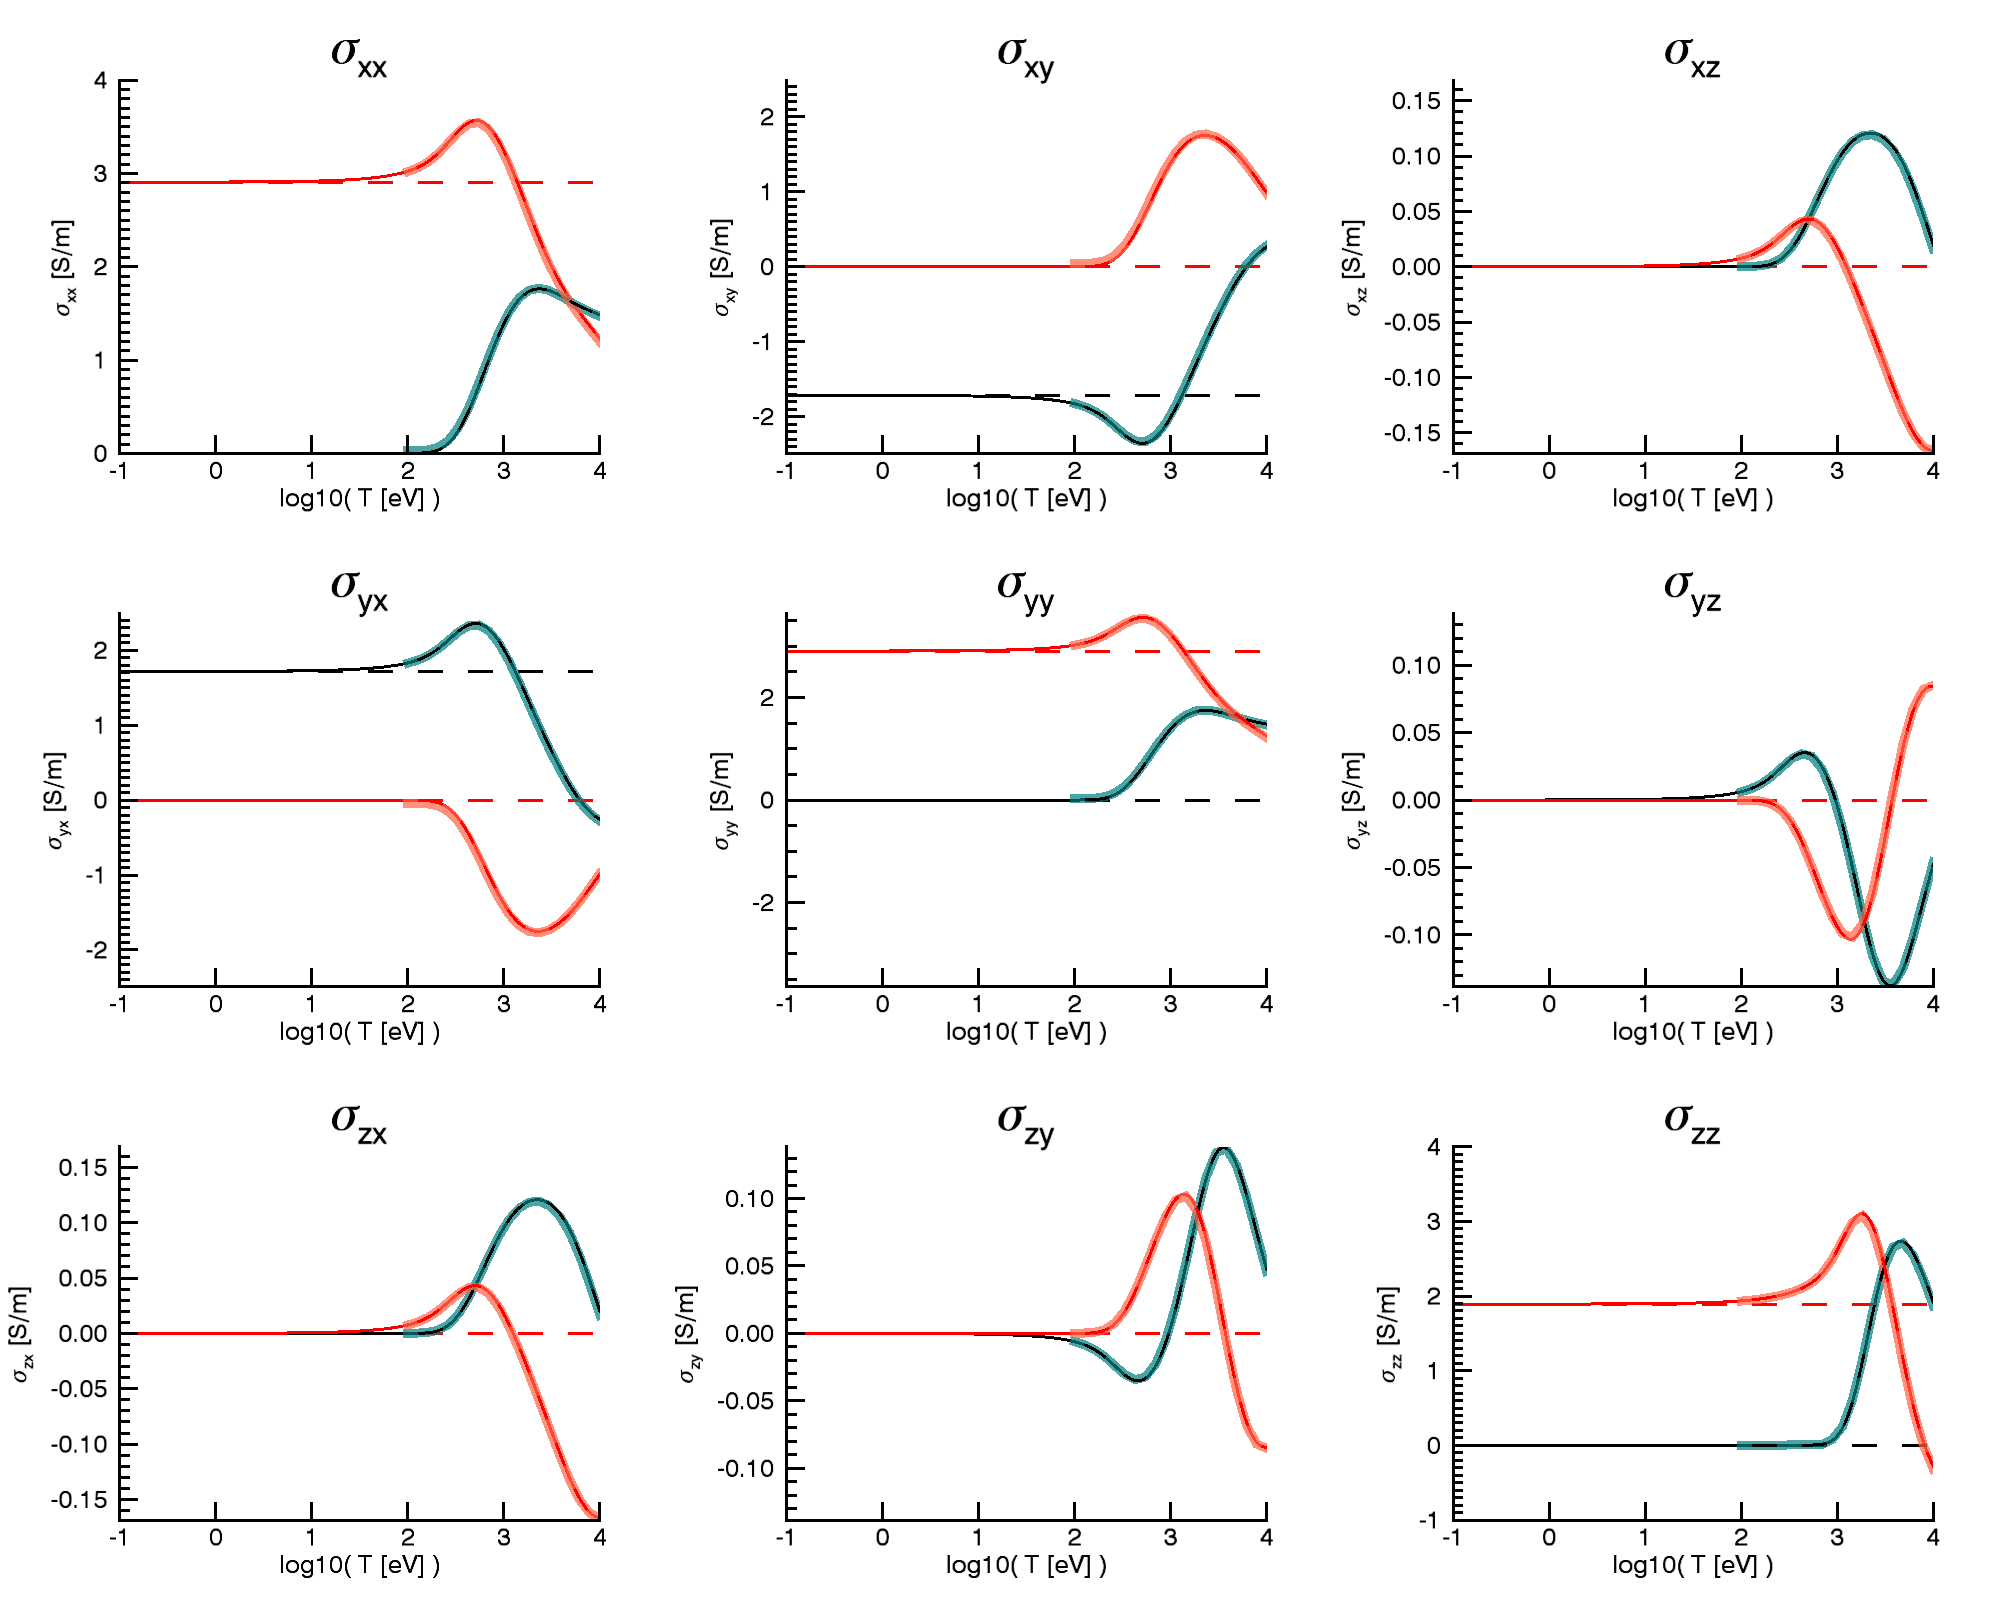
\includegraphics[]{figures/benchmark1}
\caption{\label{fig:b1}The nine components of the plasma conductivity for a range of temperatures. Black is real, red is imaginary. Cold-plasma values are shown as dotted lines for reference. The reference curves (thin, solid) are calculated separately from both the expressions in \cite{brambilla} and \cite{swanson} to provide an additional verification (and lay on top of each other such that you only see single real and imaginary reference curves). \kj calculated values are the transparent thicker curves.}
\end{figure*}
%
\subsection{Benchmark 2: $\sigma_i\left(T\right), k_{y}\ne 0$, 13 MHz}
\label{section:verification2}
%
Next we run the same case (with the same parameters), but with $k_{\mathrm{y}}\ne 0$. Here we choose $k_{\mathrm{y}}=23$ m$^{\mathrm{-1}}$. Fig.~\ref{fig:b2} shows the results, again with \kj showing agreement to the analytic expressions of \cite{swanson}.
%
\begin{figure*}
\centering
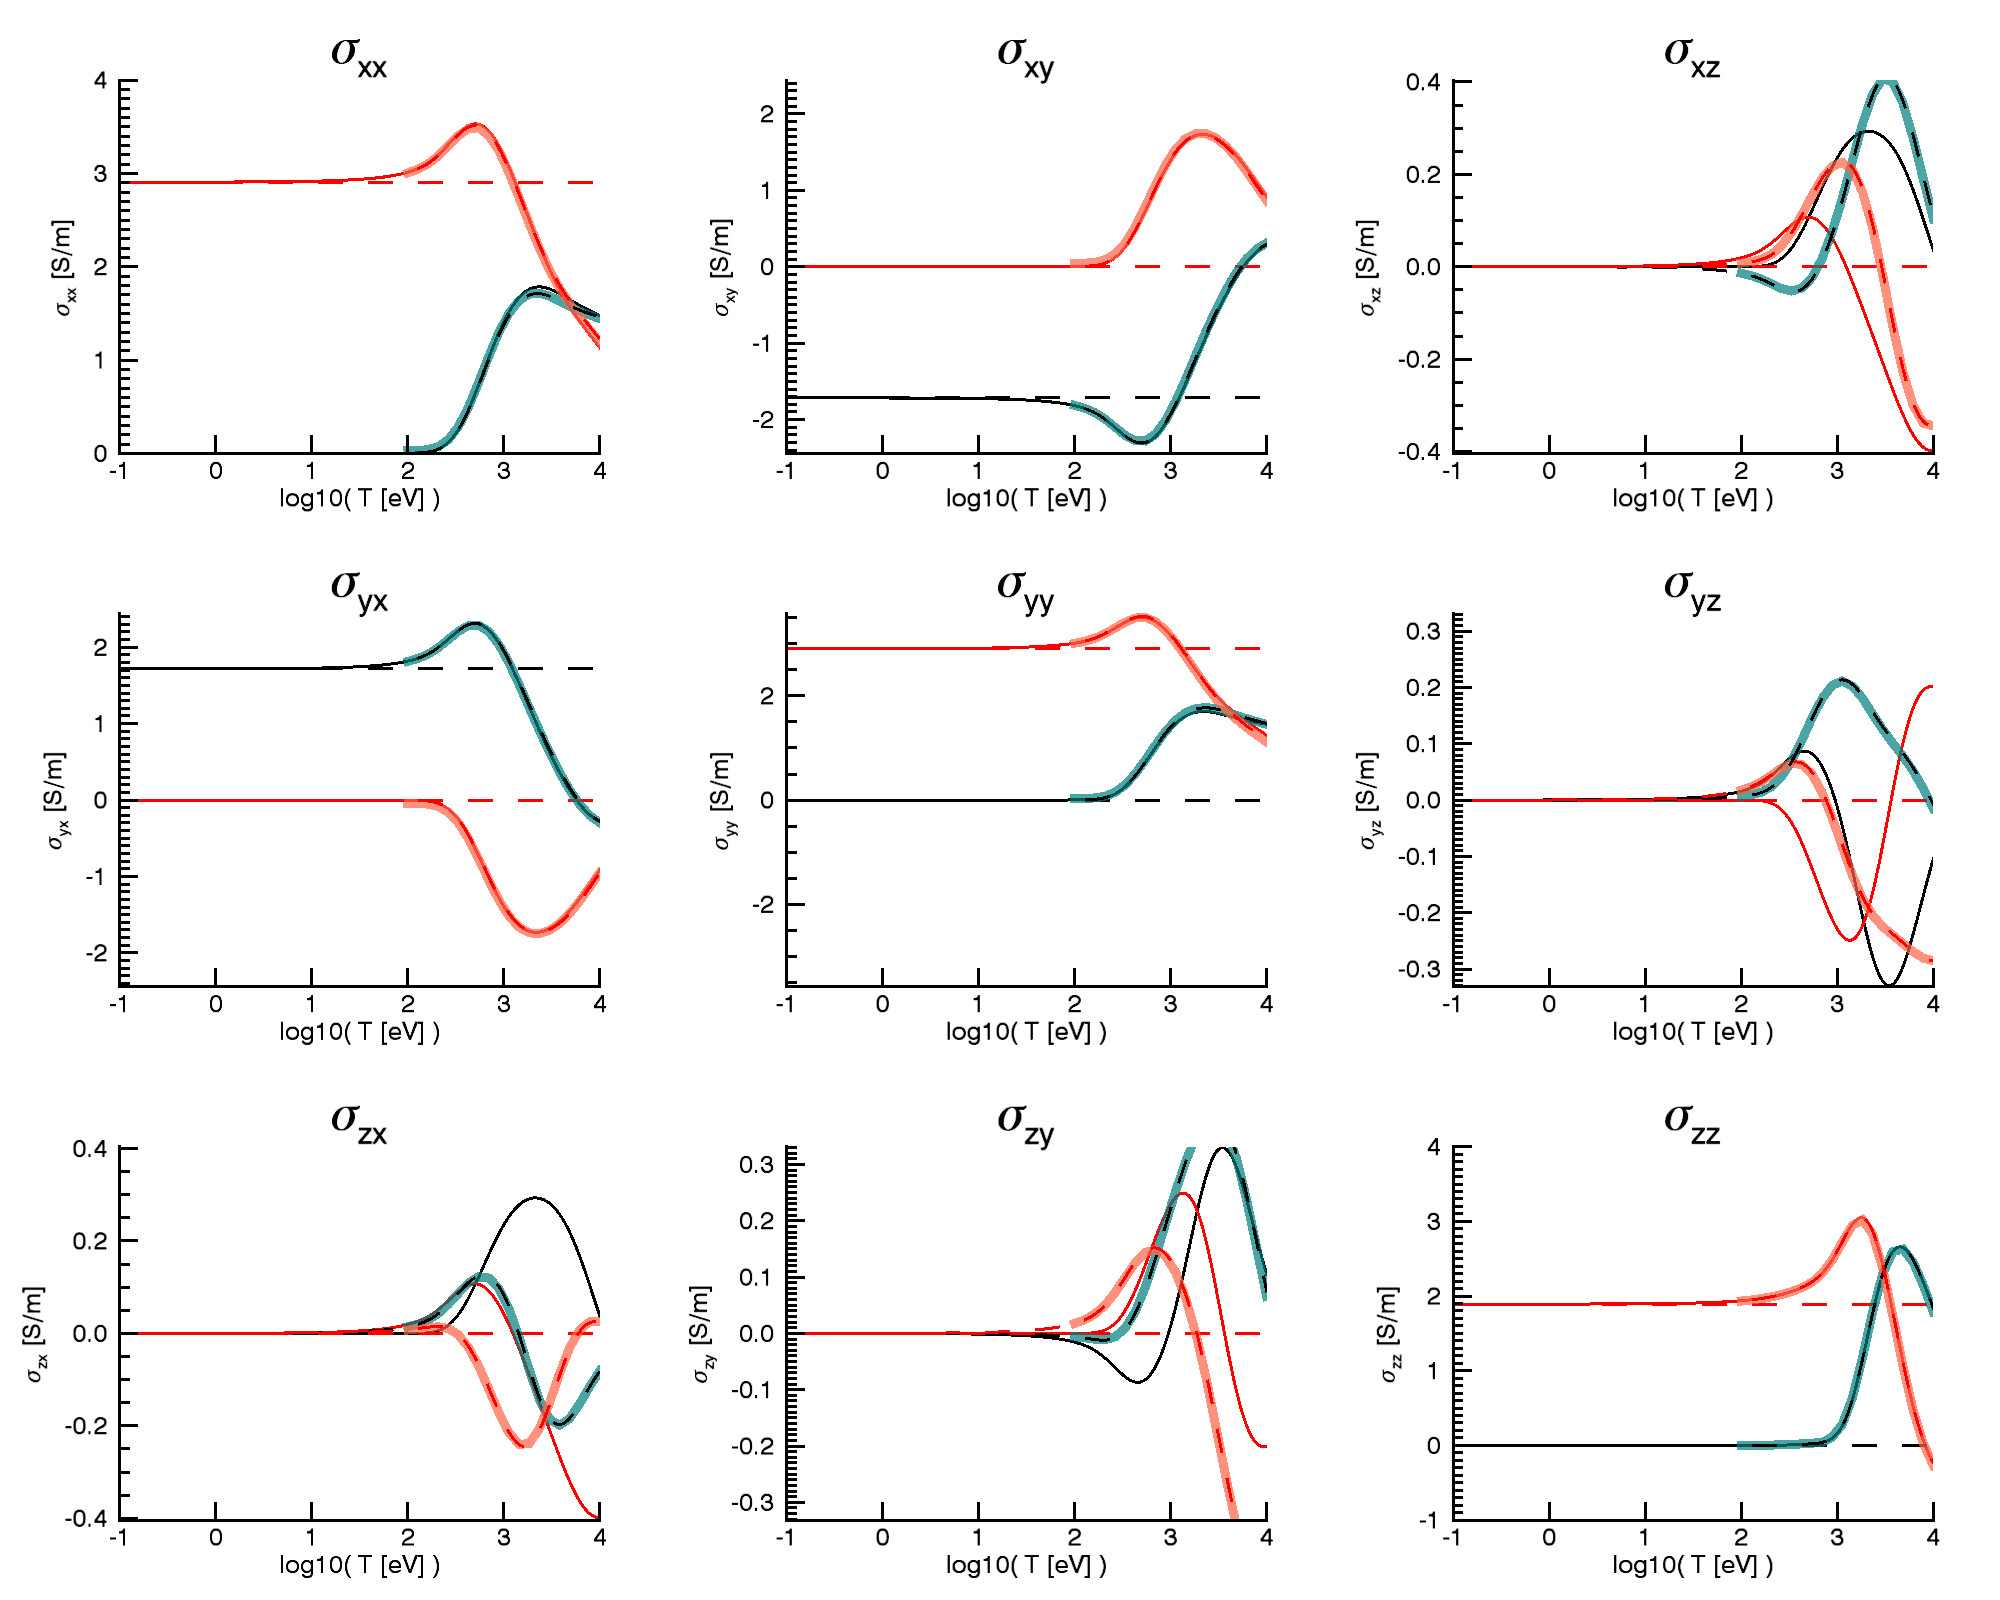
\includegraphics[]{figures/benchmark2}
\caption{Similar to Fig.~\ref{fig:b1}, but here the thin reference curves calculated from both the expressions in \cite{brambilla} (solid) and \cite{swanson} (dotted) do not overlap due to the expressions from \cite{brambilla} not including the $k_{\mathrm{y}}\ne 0$ explicitly, such that they merely reproduce the curves of Fig.~\ref{fig:b1}.}
\label{fig:b2}
\end{figure*}
%

\subsection{Benchmark 3: $\sigma_e\left(B\right)$, 32 GHz, Cyclotron Resonance}
\label{section:verification3}
%
The third benchmark case is for electrons, and is a scan over magnetic field strength such that we cover the fundamental electron cyclotron resonance at 32 GHz. The $k$ component values are those used for benchmark 1, as is the density. The parameters required here were \texttt{nThermal=3, nP\_Vx=11, nP\_vY=11, nP\_vZ=15, nRFCycles=100, nStepsPerCyclotronPeriod=100}.
%
\begin{figure*}
\centering
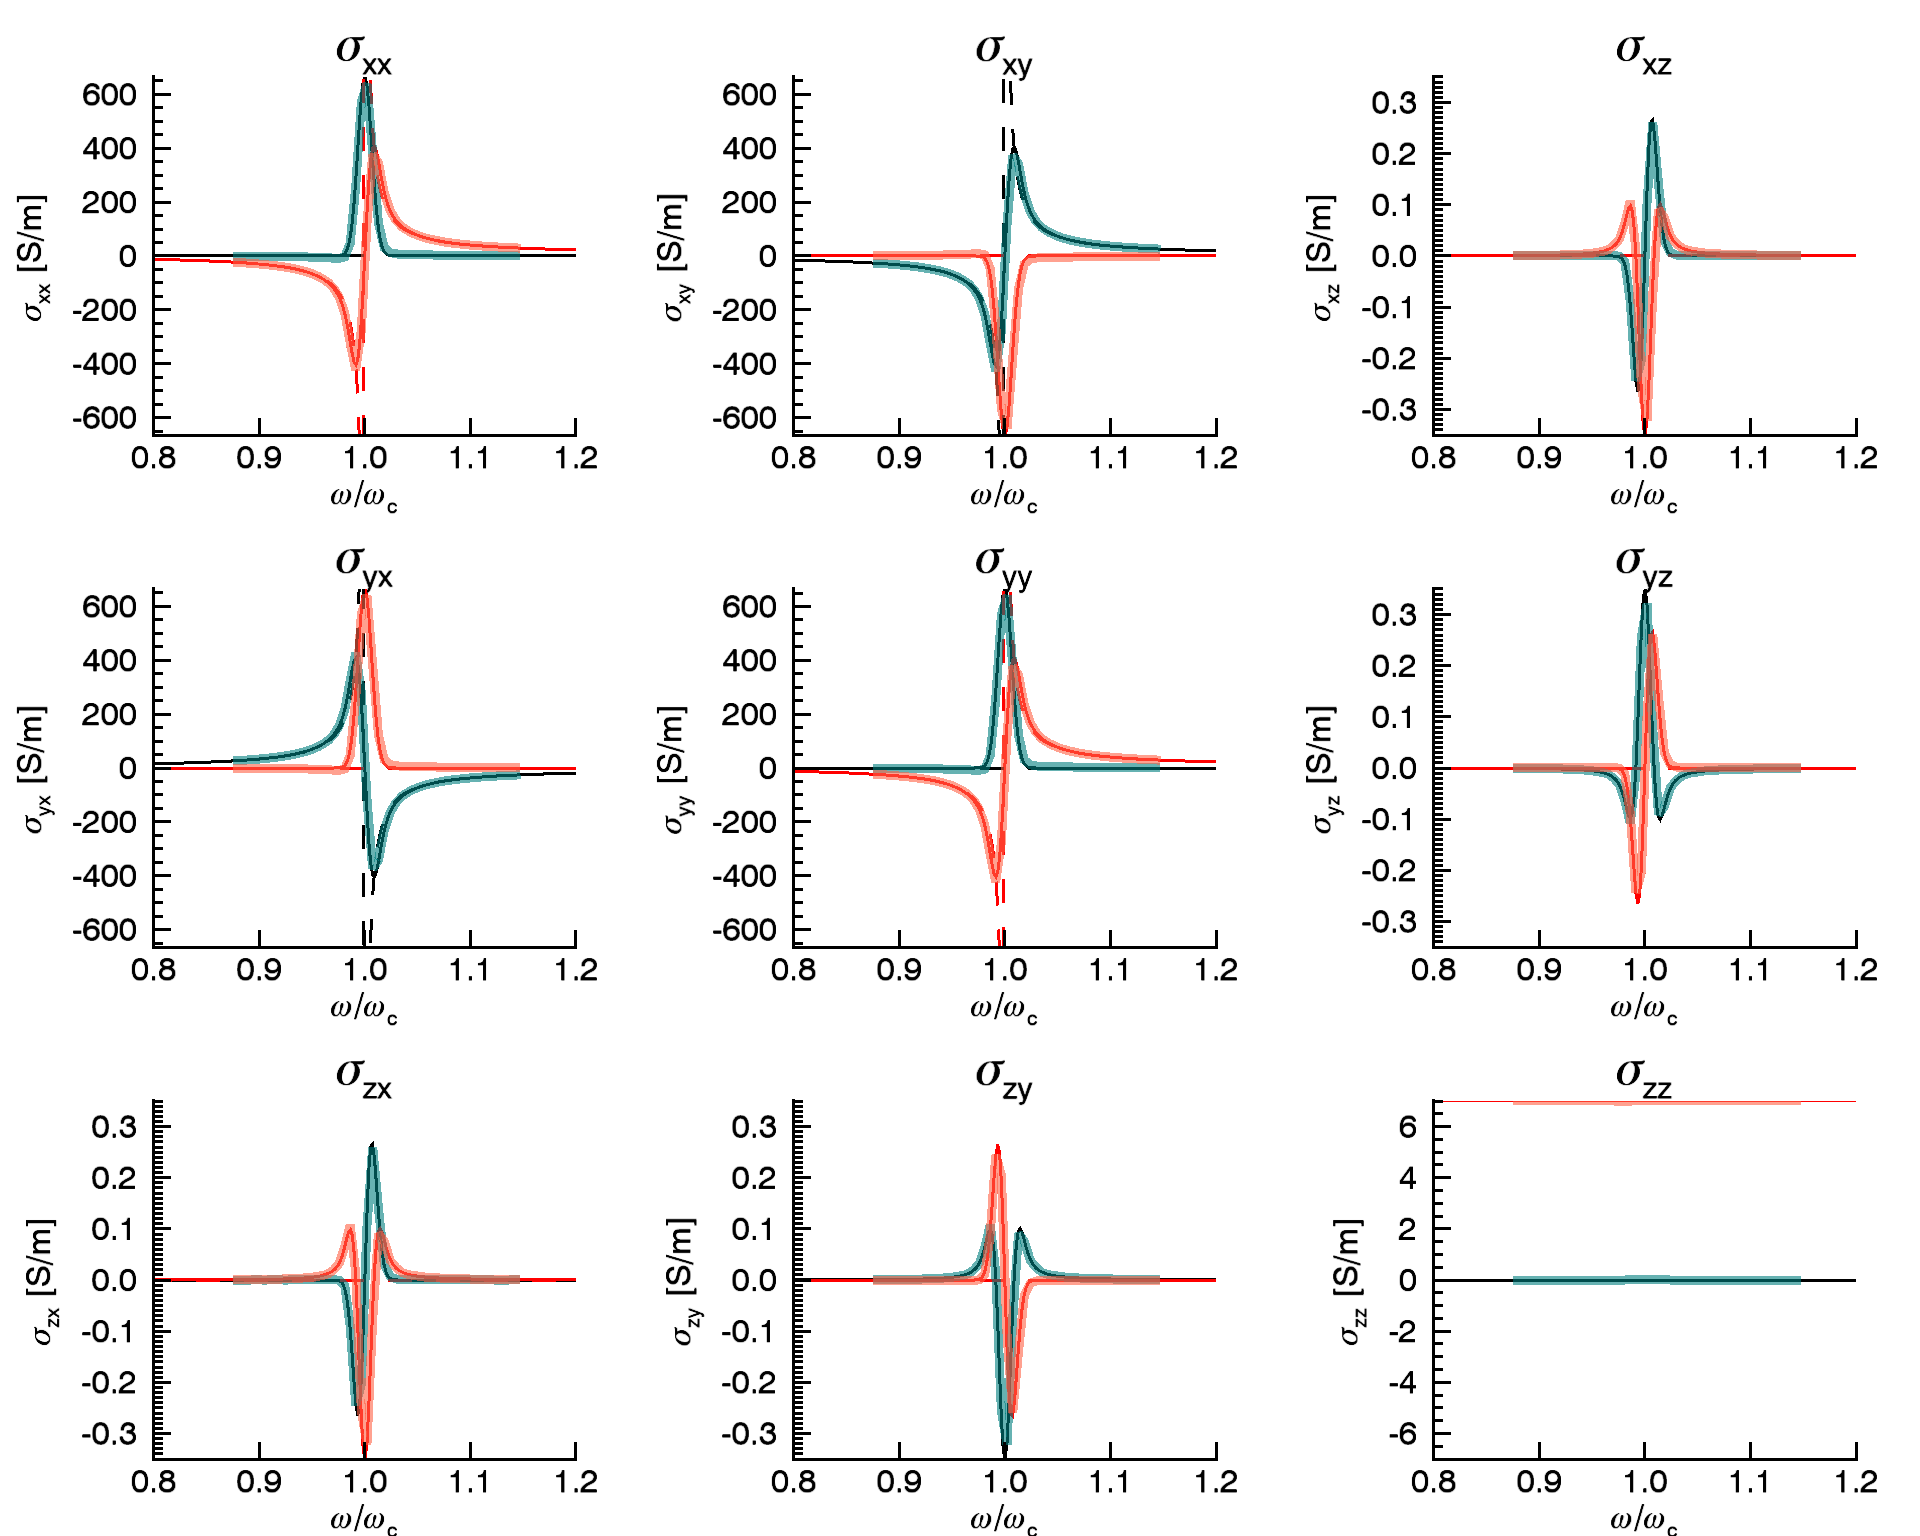
\includegraphics[]{figures/benchmark3}
\caption{Benchmark 3 results, being elements of the conductivity tensor for electrons as a function of magnetic field strength spanning the fundamental electron cyclotron resonance. As with Fig.~\ref{fig:b1}, black is real, red is imaginary. Cold-plasma values are shown as dotted lines for reference. The reference curves (thin, solid) are calculated separately from both the expressions in \cite{brambilla} and \cite{swanson} to provide an additional verification (and lay on top of each other such that you only see single real and imaginary reference curves). \kj calculated values are the transparent thicker curves spanning one a portion of the domain.}
\label{fig:b3}
\end{figure*}
%

\subsection{Choice of parameters}
\label{section:parameters}
%
The evaluation of Eqns.\ref{eq:j1} through \ref{eq:trajectories} requires several discretization parameters to be chosen. The innermost of these are the time step (controlled by \texttt{nStepsPerCyclotronPeriod} - the number of time steps per cyclotron period at the particle starting location)  and the length of the RK4 unperturbed trajectory integration (controlled by \texttt{nRFCycles} - number of RF periods). Normally one would set the time step solely by the orbit integration accuracy requirements, i.e., some number of points per cyclotron period (hence the input parameter name). However, there is also the sampling of the wave electric field to consider. In the case where an unperturbed trajectory travels into a phase front incident from the opposing direction there may be a sufficiently large Doppler shift in the observed RF frequency by the trajectory such that the Doppler shifted RF frequency sets the minimum time step. This mainly applies to the parallel direction where trajectories at sufficiently large parallel velocities encounter a wave phase velocity of opposite parallel sign with small enough $k_{\parallel}$. A useful time step can be chosen as 
%
\begin{linenomath}
\begin{equation}
\begin{split}
\label{eq:min_dt}
\Delta t=\mathrm{min}\Bigg(\frac{2\pi}{\omega_c\texttt{nPtsPerCyclotronPeriod}} ,\\ \left(1+\frac{\texttt{nThermal}v_{\mathrm{th}}}{\vec{v}_{\mathrm{p}}\cdot\hat{\vec{B}}}\right)f_{\mathrm{RF}}\times\texttt{nPtsPerCyclotronPeriod}\Bigg)
\end{split}
\end{equation}
\end{linenomath}
%
where $\vec{v}_\mathrm{p}$ is the global minimum of the phase velocity of the wave electric field and $v_{\mathrm{th}}$ is the thermal velocity of the Maxwellian distributions.  

In our benchmark cases, increasing the length of the time integral (controlled by \texttt{nRFCycles}) converges the \kj solution to the analytic result. However, it also sharpens the velocity space features of $f_\mathrm{1}$, which then couples \texttt{nRFCycles} to the velocity space resolution, i.e., as \texttt{nRFCycles} is increased, the sampling of velocity space also needs to increase to avoid under sampling the increasingly fine features and producing errors in the current. Here we uniformly sample velocity space in Cartesian coordinates with the range of velocity space being the same in all directions, set to $[-\texttt{nThermal}\times v_{\mathrm{th}},+\texttt{nThermal}\times v_{\mathrm{th}}]$ and grid resolutions in each direction controlled by \texttt{nP\_Vx}, \texttt{nP\_Vy}, and \texttt{nP\_Vz}. 

Parameter selection, particularly the velocity space sampling, is an important aspect of running \kj, but it also has a strong impact on the run time required. The parameters are problem dependent, and at present convergence is reliant upon checking sensitivity to these choices and the operator to understand where resolution and sampling may be required, and what the symptoms are of choosing sub-optimal parameters. While adaptive sampling methods are an attractive choice, for the present work we have retained uniform step size and meshing to enable ease of programming for GPU architectures, thus enabling reasonable wall-clock times. An area of future work will be algorithm development to enable GPU implementation of  adaptive velocity space sampling, and / or trajectory (and subsequent $\vec{E}_{\mathrm{1}}$, Doppler shifted, sampling) time stepping.

\section{Performance}
\label{section:performance}
%
The configuration space evaluation of Eqns.\ref{eq:j1}-\ref{eq:trajectories} is extremely expensive when compared to evaluation of the analytic expressions of \cite{stix}. However, we have to keep in mind that the goal here is improved algorithmic scaling (work required as a function of degrees of freedom) to solve the larger linear, kinetic full-wave problem presented in \cite{green2014}. As such, we target GPU based architectures for acceleration of the \kj kernels. This is achieved by utilizing the CUDA\footnote{\url{https://developer.nvidia.com/cuda-toolkit}} THRUST library\footnote{\url{https://developer.nvidia.com/thrust}}. The use of the parallel execution policies within THRUST further provide us a serial CPU and OpenMP parallel execution options with no changes to the code by the choice of the compile time execution policy (\texttt{-DTHRUST\_DEVICE\_SYSTEM = THRUST\_DEVICE\_SYSTEM\_\$TARGET} where \texttt{\$TARGET} is one of \texttt{"CPP"} for serial, \texttt{"OMP"} for OpenMP parallel implementation, and \texttt{"CUDA"} for the GPU implementation). The parallelization worklist is over the 4D space consisting of a single spatial coordinate (only a single point in these benchmark scans) and 3 velocity coordinates. Figure~\ref{fig:scaling} shows the run time for a single \kj run for increasing velocity space resolution. We show curves for serial, OpenMP with 24 threads, and a single GPU. The NVIDA Tesla (Kepler) K80 card we use has 4992 CUDA cores, which are only effectively utilized near the 1 million threads level. All calculations are single precision. The results of Fig.~\ref{fig:scaling} show a speedup of $\sim$3x at 1 million work list elements over full OpenMP utilization of the 24 available CPUs on the single node utilized here. This included $\sim$10\% time for copying the data to and from the GPU.  
%
\begin{figure}
\centering
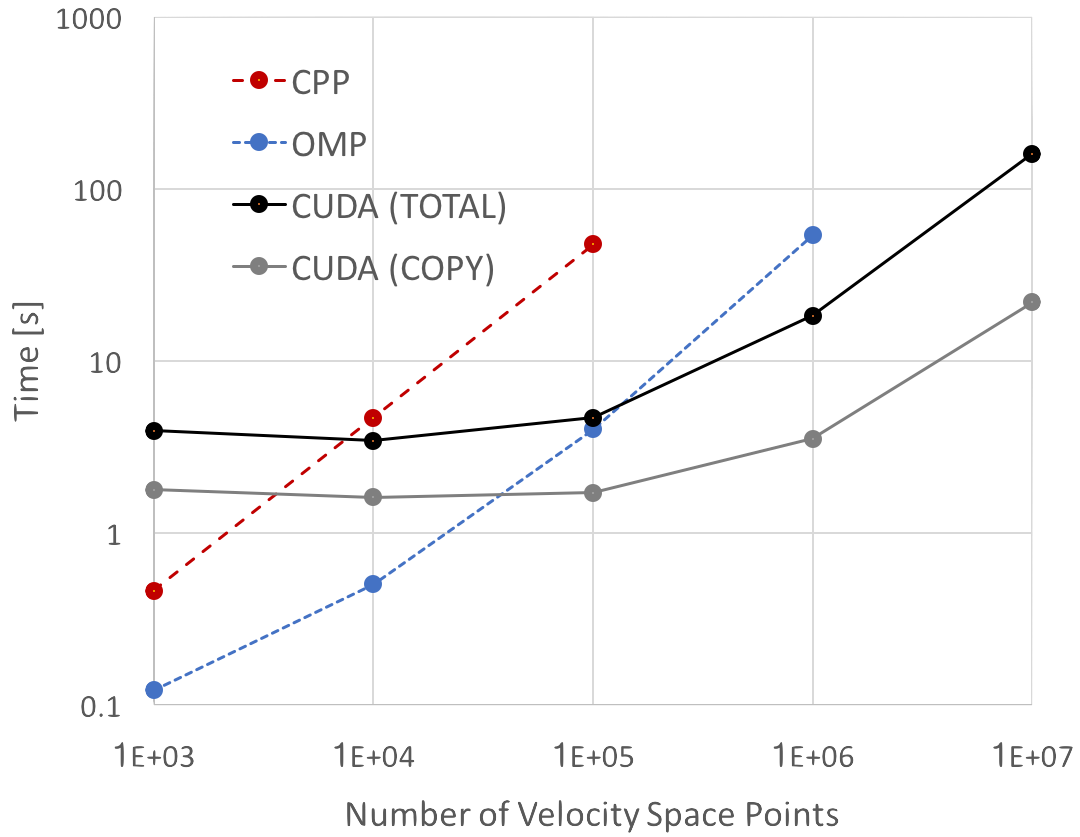
\includegraphics[width=0.5\textwidth]{figures/scaling}
\caption{Performance for serial CPU, OpenMP, and GPU implementations using the THRUST library parallel execution policy such that no code changes are required for the different curves.}
\label{fig:scaling}
\end{figure}
%
\section{Discussion and Future Work}
\label{section:discussion}
%
We have presented a computational kernel for evaluating the linear kinetic plasma current for an arbitrary time-harmonic electric wave field. The intended use case is within a larger iterative operator-split approach to solving 2 and 3-D kinetic full-wave problems for RF heating and current drive in fusion plasmas as presented in \cite{green2014}. Three benchmark cases confirm \kj is able to reproduce the analytic solution for simple, single $\vec{k}$ uniform wave fields. While the uniform velocity space sampling and fixed time stepping for the trajectory integrations yield satisfactory results, we identify the robust and automatic / adaptive non-uniform velocity space sampling and time stepping as a future goal to reduce the computational overhead. 
%
\section{Acknowledgements}
\label{section:acknowledgements}
This research used resources of the Oak Ridge Leadership Computing Facility at the Oak Ridge National Laboratory, which is supported by the Office of Science of the U.S. Department of Energy under Contract No. DE-AC05-00OR22725.


%% The Appendices part is started with the command \appendix;
%% appendix sections are then done as normal sections
%% \appendix

%% \section{}
%% \label{}

%% References
%%
%% Following citation commands can be used in the body text:
%% Usage of \cite is as follows:
%%   \cite{key}         ==>>  [#]
%%   \cite[chap. 2]{key} ==>> [#, chap. 2]
%%

%% References with bibTeX database:

\bibliographystyle{elsarticle-num}
\bibliography{fusion}

%% Authors are advised to submit their bibtex database files. They are
%% requested to list a bibtex style file in the manuscript if they do
%% not want to use elsarticle-num.bst.

%% References without bibTeX database:

% \begin{thebibliography}{00}

%% \bibitem must have the following form:
%%   \bibitem{key}...
%%

% \bibitem{}

% \end{thebibliography}


\end{document}

%%
%% End of file 
